%! Author = tstreule

\section{PET \textnormal{-- Positron Emission Tomography}}

\begin{minipage}{.2\linewidth}
    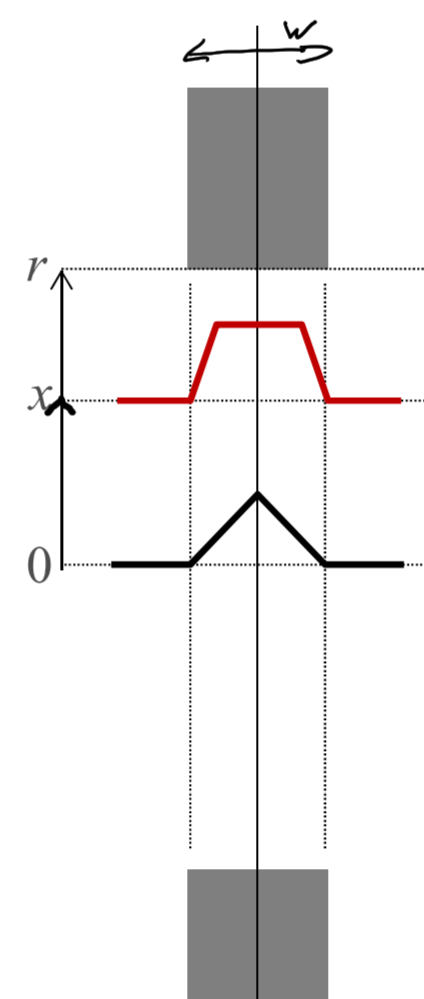
\includegraphics[width=.9\linewidth]{PET_PSF}
\end{minipage}
\begin{minipage}{.8\linewidth}
    \textbf{Positron range} $\propto$ E. \quad $\textrm{FWHM}\approx 0.1 - 0.5 \unit{mm}$.

    \textbf{Radionuclide}: $\ce{^{18}F}$ better than $\ce{^{11}C}$ (110 vs 20 min)

    \textbf{Image production}: Scintillator (fine grid) $\to$ PMT / avalance Diode $\to$ Electronics. Event finding in scintillator is linear.
    \fbox{$y = \frac{ S\ped{A}+S\ped{B}-S\ped{C}-S\ped{D} }{ S\ped{A}+S\ped{B}+S\ped{C}+S\ped{D} }$}

    \textbf{PSF}: Trapezoid/Triangle. \highlight{$\displaystyle \textrm{FWHM} = w\frac{r+x}{2r}$}\\
    {\scriptsize r: Ring diameter, x: distance from center, w: grid spacing of sc.}
\end{minipage}
%%%%%%%%%%%%%%%%%%%%%%%%%%%%%%%%%%%%%%%%%%%%%%%%%%%%%%
\subsection{Efficiency (to actually measure concentrations)}
Detection eff. $\epsilon = (1-e^{-\mu d}) \cdot \Phi$ \hfill ($\Phi$: frac. of events in E window)

Geometric eff.: $\Omega = 4\pi \sin(\arctan(z/D))$ \hfill $D=2r$, $z$: length

Radial geometric coverage $\phi$: Fraction not gap between crystals

\textbf{Total sensitivity}: \highlight{$\displaystyle \eta = \epsilon^2 \phi \frac{\Omega}{4\pi}$}
%%%%%%%%%%%%%%%%%%%%%%%%%%%%%%%%%%%%%%%%%%%%%%%%%%%%%%
\subsection{Problems, solutions and additions}
\textbf{Correction table} for which scintillator under PMT

\textbf{Correction matrix}: against non-uniform detector eff.

\textbf{Attenuation correction}: Measure Image in HU via X-Ray CT, $\to$ attenuation coeff. $\to$ multiply PET lines by $\eu^{\mu D_{ij}}$

\textbf{Random coincidence}: Measure Background noise, then -

\textbf{Detector dead time} $\delta$: $N\ped{measured} = N\ped{true} \eu^{-N\ped{true} \delta}$

\textbf{TOF} (Time Of Flight of photon): $\Delta x = \frac{c\Delta t}{2} = \unit[75]{mm} \;\widehat{=}\; \unit[500]{ps}$

\textbf{3D image reconstr.}: Use coinc. between different rings.
%%%%%%%%%%%%%%%%%%%%%%%%%%%%%%%%%%%%%%%%%%%%%%%%%%%%%%
\subsection{Quantitative PET - various effects and definitions}
\textbf{Partial voluming}: When measuring the \underline{intensity} of an object, it appears smaller at the edge of the object than it is. $\to$ Only measure in the center

\textbf{Injected dose per gram of tissue} \fbox{$\%ID/g = \frac{c_t v_t}{D_{inj}} \cdot \frac{1}{m_t} \cdot 100\%$}, \quad
$c_t$: tissue conc., $v_t$: vol. of tissue ROI, $m_t$: mass of tissue ROI, $D\ped{inj}$: injected dose

\textbf{Standardized uptake value} ($M$: Body mass, $S$: surface)\\
\highlight{$\displaystyle SUV = [\%ID/g] \cdot M/100$} \highlight{$\displaystyle SUV' = [\%ID/g] \cdot S / 100$}

\textbf{Distribution volume}: Volume of blood needed for $M$ \#tracer.\\
\fbox{$V_d = M/c_b = V_t c_t/c_b + V_b = V_t \lambda + V_b$} \quad $\lambda =  c_t/c_b$\\
$V_t \lambda = V_1$ = equiv blood vol. to tissue vol. where tracer is\\
$c_b$: typ. conc. of that tracer in blood. $V_d > 7 \ell \implies$ body.
%%%%%%%%%%%%%%%%%%%%%%%%%%%%%%%%%%%%%%%%%%%%%%%%%%%%%%
\subsection{The scatchard equation}
\textbf{\underline{L}igand} (tracer/drug), \textbf{\underline{R}eceptor}. \quad Reaction: L+R = RL

$[L], [R], [RL]$: conc. ---
$[R_T]$: total \#receptors ---
$k\ped{off}, k\ped{on}$: reaction rates ---
$k\ped{off} \cdot [RL]$: \#bound pairs that separate.

Equilibrium eq.: $k\ped{off} \cdot [RL] = k\ped{on} \cdot [R] \cdot [L]$ \\
Eq. const.: $K_d = \frac{k\ped{off}}{k\ped{on}} = \frac{[R] \cdot [L]}{[RL]}$ \hfill
\highlight{$\displaystyle \frac{[RL]}{[L]} = -\frac{1}{K_d} \cdot [RL] + \frac{R_T}{K_d}$}\\
Scatchard plot: $\textrm{slope} = 1/K_d$, $R_T$: intersection with $[RL]$-axis
%%%%%%%%%%%%%%%%%%%%%%%%%%%%%%%%%%%%%%%%%%%%%%%%%%%%%%
\subsection{Kinetic models}
\textbf{Renking-Crone eq.}: (amount of substance diffuses out of a blood capillary)\\
\highlight{$\displaystyle = F \cdot E$} \highlight{$\displaystyle E = 1 - \eu^{-P \cdot S / F}$}
$E$: Efficiency, $P$: vascular permeability, $S$: capillary surface, $F$: blood flow

\textbf{Kinetic model}: ($c_p$: Plasma $\leftarrow$ particular part)\\
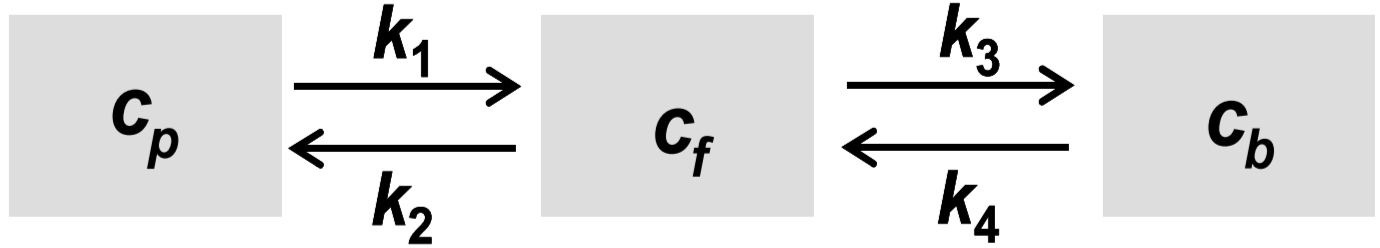
\includegraphics[width = 0.45\linewidth]{PET_Kinetic_Model}
$c_f$: free ligands, $c_b$: bound l

\textbf{Kin. eq.}:
$\deriv{c_f}{t} = k_1 c_p - (k_2 + k_3) c_f + k_4 c_b$, \;---\;
$\deriv{c_b}{t} = k_3c_f - k_4c_b$, \;---\;
$k_1 = FE$, \;---\;
$k_2 = k_1 c_p/c_f$, \;---\;
$k_3 = k_{on} [R]$, \;---\;
$k_4 = k_{off}$

What is measured: $c_t(t) = c_f(t) + c_b(t)$. $* c_p(t)$ should be in the equation. $\to$ At the end determine the rate constants.

\textbf{Improvement}: Look at reference section in brain without receptors. Only 2 compartment model, measure $k_1$ and $k_2$.

To measure behaviour of a drug (cold): Tracer (hot) $\to$ same receptors. Experiment with and without drug. Assumption: $c_b << c_{b,d}$. The drug changes the \# total receptors from $B_{max}$ to $B'_{max}$. \textbf{Receptor occupancy for drug}:\\
\fbox{$\textrm{RO}[\%] = \frac{c_{b,d}}{B\ped{max}} = (1 - B'\ped{max}/B\ped{max})\cdot 100\%$}
